\section{API Design}

To ensure consistency with industry standards and facilitate efficient collaboration, the system adopts the OpenAPI Specification (version 3) to define and document all developed APIs. Based on this specification, the Swagger interface is integrated into the backend service, providing an interactive environment where developers and clients can explore, test, and understand the available endpoints.

As illustrated, the Swagger UI serves as a centralized and up-to-date documentation platform, allowing developers and integrators to quickly access API details such as request parameters, response formats, and authentication requirements. This approach significantly improves development efficiency, reduces integration complexity, and ensures better communication between frontend and backend components.

\begin{figure}[h!]
    \centering
    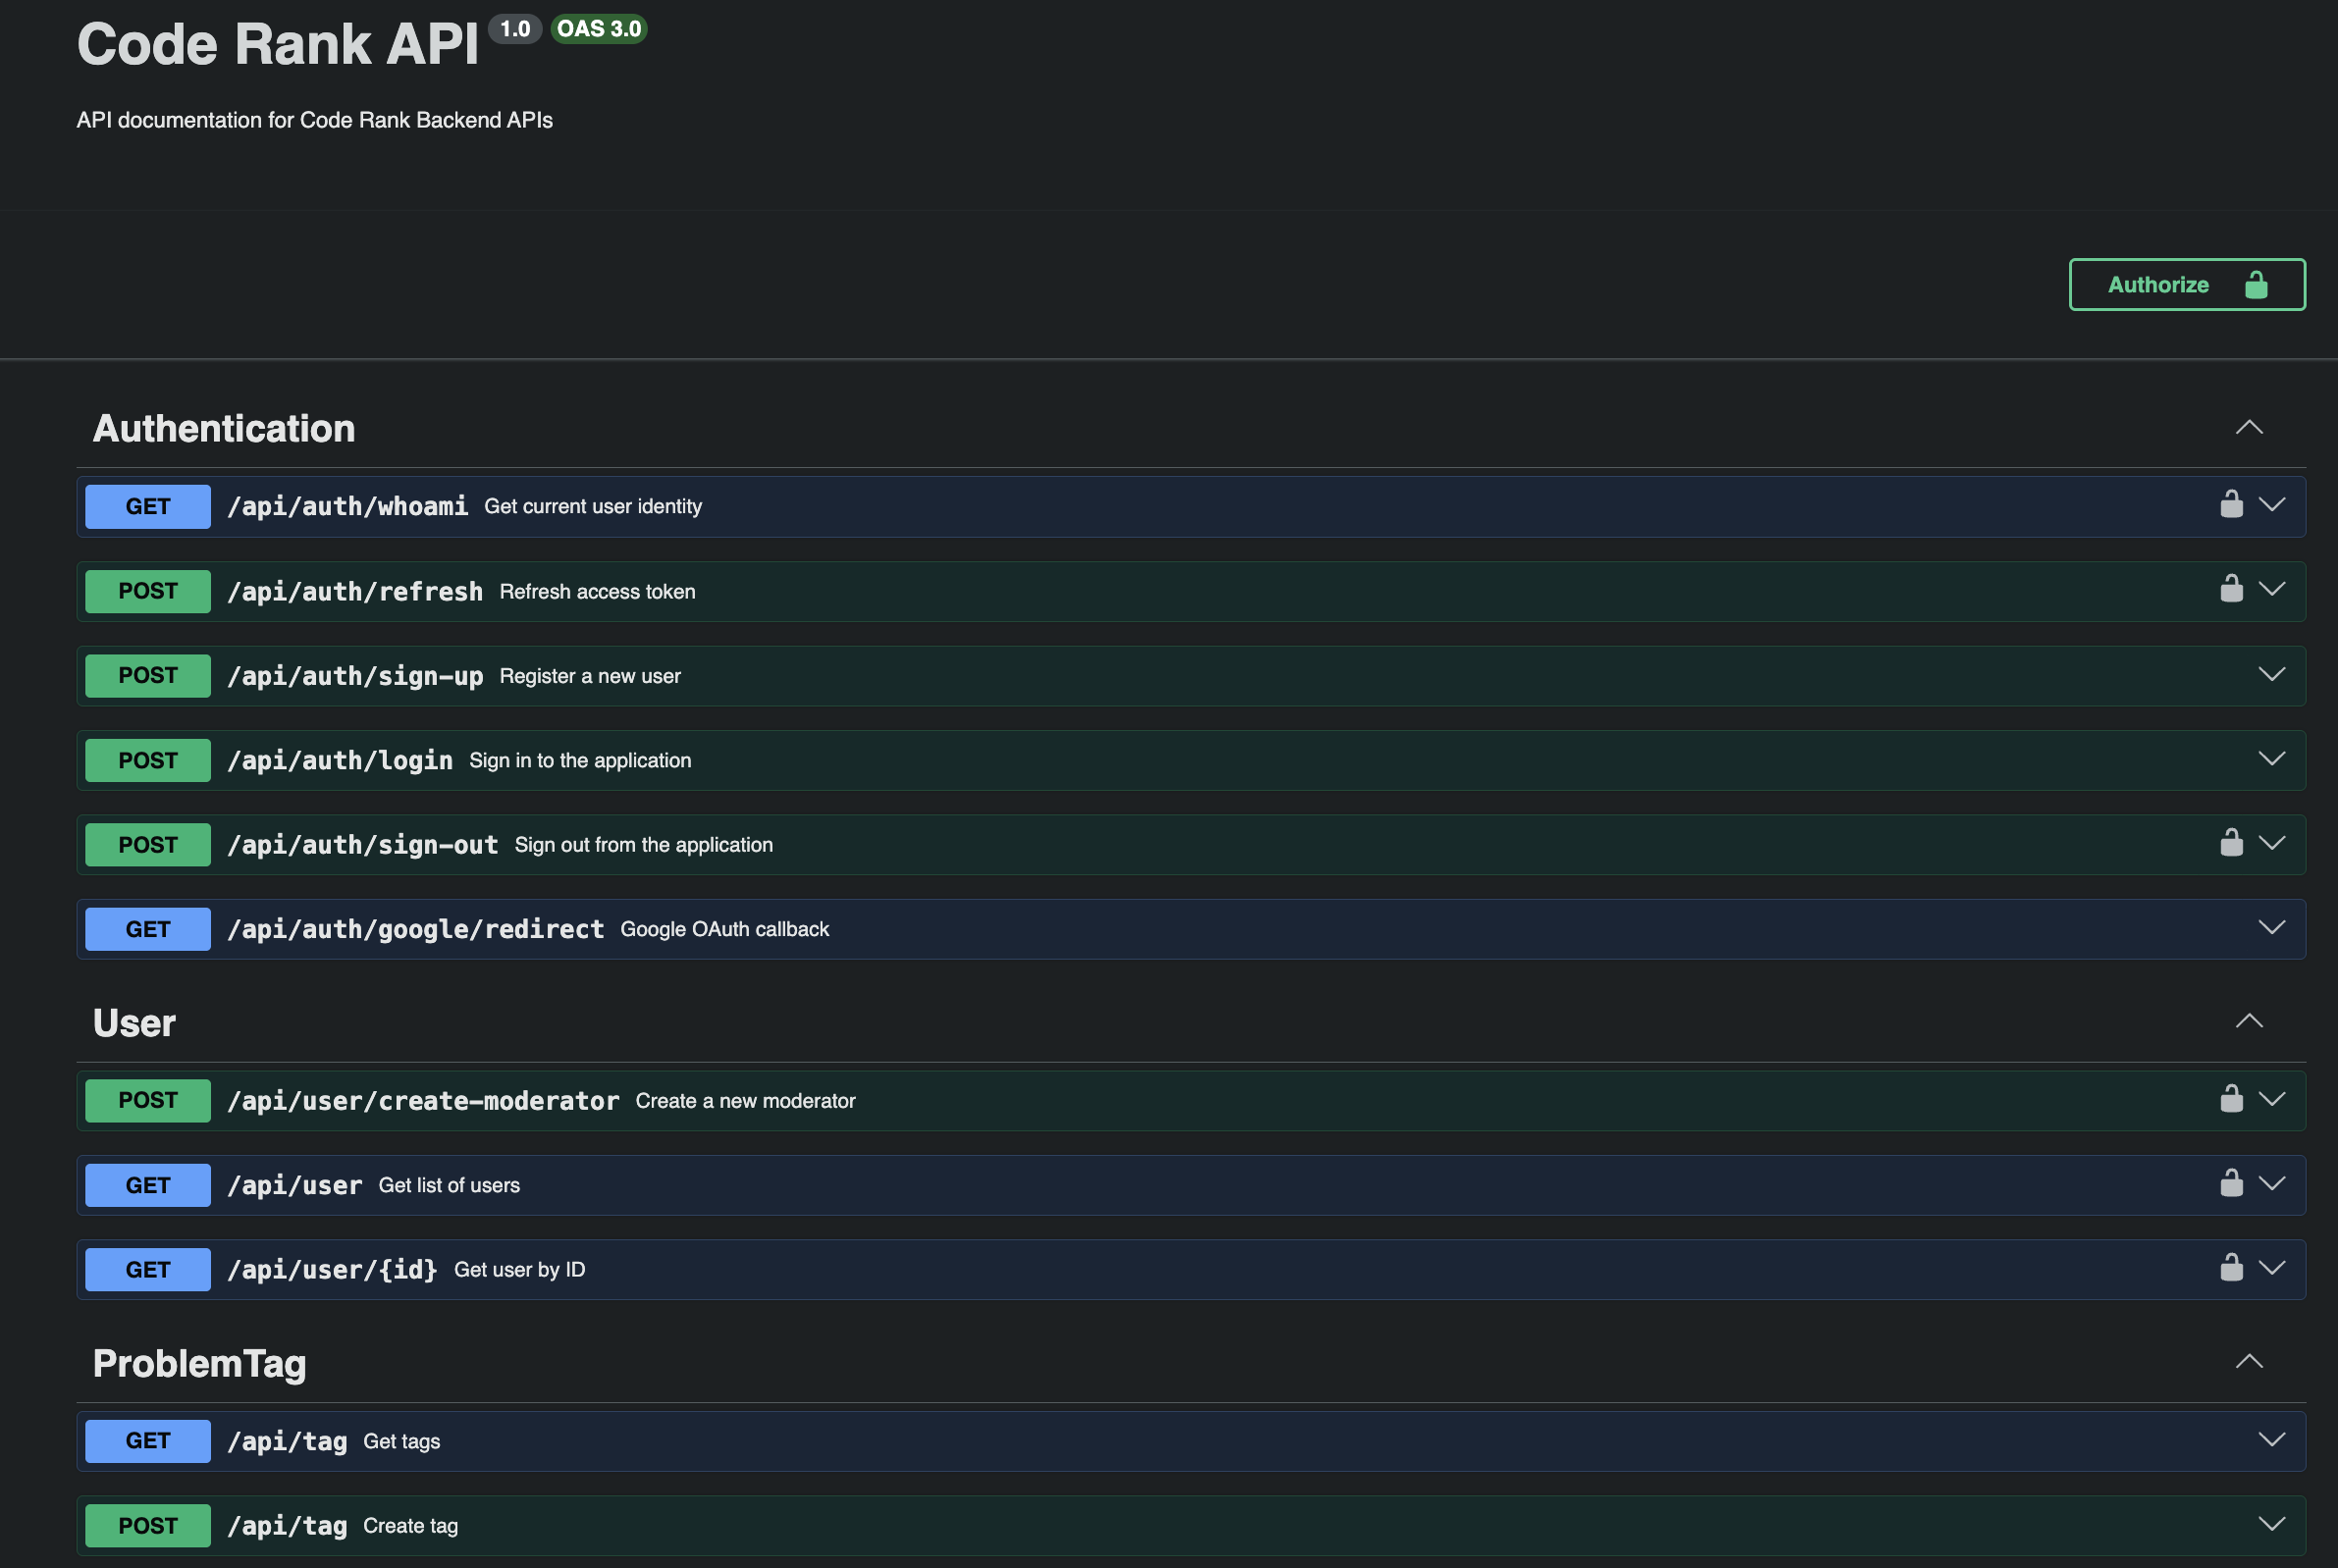
\includegraphics[width=1\textwidth]{Contents/Chapter 4/API Design/SwaggerApi.png}
    \vspace{0.6cm}
    \caption{API Swagger}
\end{figure}

\break